

\documentclass[8pt, usepdftitle = false]{beamer}
% \imput{../common/beamerthemesimple}
\usetheme{simple}


  \usepackage{xcolor}
  \definecolor{olive}{rgb}{0.3, 0.4, .1}
  \setbeamercolor{itemize/enumerate body}{fg=black}
  \setbeamercolor{title}{fg = green!30!black}
  \setbeamercolor{frametitle}{fg = gray!70!black, bg = white}


% \usepackage{lmodern}
\usepackage[scale = 2]{ccicons}
\usepackage[export]{adjustbox}
\usepackage{amsmath, amsthm, amssymb}
\usepackage{amsfonts}
\usepackage{mathtools}

\usepackage[justification=raggedright,width=\linewidth]{caption}
\usepackage{tikz} 


\usepackage{setspace}

\setbeamertemplate{title page}[default][right,colsep=-4bp,rounded=true,shadow=\beamer@themerounded@shadow]

\setbeamertemplate{caption}[numbered]


%% Options

\setbeamercolor{alerted text}{fg=blue}
\setbeamertemplate{alerted text begin}{\itshape}
\setbeamertemplate{alerted text end}{}

\newenvironment<>{varblock}[2][\textwidth]{%
    \setlength{\textwidth}{#1}
    \begin{actionenv}#3%
        \def\insertblocktitle{\underline{#2}}%
        \par%
        \usebeamertemplate{block begin}}
        {\par%
        \usebeamertemplate{block end}%
    \end{actionenv}}

\setbeamertemplate{blocks}[rounded][shadow=true]
\setbeamercolor{block title}{fg=black,bg=gray!20!white}
\setbeamercolor{block body}{fg=black,bg=gray!10!white}




%% Theorem

% \newtheorem{theorem}{Theorem}

%% Bangla tex


\usepackage{polyglossia}
\setotherlanguage[numerals=Devanagari]{bengali}
\setmainlanguage{english}
\newfontfamily\bengalifont[Script=Bengali]{Akaash}


%% tikx

\usepackage{tikz}
\usetikzlibrary{calc,trees,positioning,arrows,fit,shapes,calc}





\newcommand\blfootnote[1]{%
  \begingroup
  \renewcommand\thefootnote{}\footnote{#1}%
  \addtocounter{footnote}{-1}%
  \endgroup
}



\newcommand\Permute[2][^n]{\prescript{#1\mkern-2.5mu}{}P_{#2}}
\newcommand\Combine[2][^n]{\prescript{#1\mkern-0.5mu}{}C_{#2}}


\renewcommand*{\thefootnote}{\fnsymbol{footnote}}


\usepackage{flexisym}
\usepackage{breqn}

\usepackage[T1]{fontenc}

% \usepackage{mathpazo}
% \renewcommand{\rmdefault}{put}

% \usepackage{fourier} 
% Only use the math font of mathpazo
% \let\temp\rmdefault
% \usepackage{mathpazo}
% \let\rmdefault\temp
% \renewcommand{\rmdefault}{put}


% \usepackage[hyphens]{url}


  % \usefonttheme{professionalfonts} % using non standard fonts for beamer
  % \usefonttheme{serif} % default family is serif

  % \usepackage{gentium}
  \usepackage{multicol}
  \usepackage{mathpazo}



% \renewcommand{\familydefault}{\sfdefault}  


  % color brackets
  \makeatletter
  \newcount\bracketnum
  \newcommand\makecolorlist[1]{%
      \bracketnum0\relax
      \makecolorlist@#1,.%
      \bracketnum0\relax
  }
  \def\makecolorlist@#1,{%
      \advance\bracketnum1\relax
      \expandafter\def\csname bracketcolor\the\bracketnum\endcsname{\color{#1}}%
      \@ifnextchar.{\@gobble}{\makecolorlist@}%
  }
  \let\oldleft\left
  \let\oldright\right
  \def\left#1{%
      \global\advance\bracketnum1\relax 
      \colorlet{temp}{.}%
      \csname bracketcolor\the\bracketnum\endcsname
      \oldleft#1%
      \color{temp}%
  }
  \def\right#1{%
      \colorlet{temp}{.}%
      \csname bracketcolor\the\bracketnum\endcsname
      \oldright#1%
      \global\advance\bracketnum-1\relax
      \color{temp}%
  }
  \makeatother


  \makecolorlist{black,blue,red}






\setbeamertemplate{section in toc}{%
  {\color{firstcolor}\inserttocsectionnumber.}~\inserttocsection}
\setbeamercolor{subsection in toc}{bg=white,fg=black}
\setbeamertemplate{subsection in toc}{%
  \hspace{1.2em}{\color{firstcolor}\rule[0.3ex]{3pt}{3pt}}~\inserttocsubsection\par}


\setbeamerfont{section in toc}{size=\fontsize{6}{8}\selectfont}
\setbeamerfont{subsection in toc}{size=\fontsize{6}{8}\selectfont}
\setbeamerfont{subsection in toc shaded}{size=\fontsize{6}{8}\selectfont}


\makeatletter
\patchcmd{\beamer@sectionintoc}{\vskip1.5em}{\vskip0.5em}{}{}
\makeatother






  \usepackage{twemojis}
  \usepackage{fontspec}
  \usepackage{tikzsymbols}
  \newfontfamily\DejaSans{DejaVu Sans}

% for R
\usepackage[fixed]{fontawesome5}


\setbeamercolor{emph}{fg=red}
\renewcommand<>{\emph}[1]{%
  {\color{purple}\only#2{\rm\itshape}#1}%
}

\setbeamertemplate{frametitle continuation}{}


\usepackage[round,  maxcitenames=10, mincitenames=11]{natbib}
\setlength{\bibhang}{0pt}
\renewcommand{\bibsection}{}
\usepackage{fancybox}


\setbeamertemplate{section page}
{
    \begingroup
    \begin{beamercolorbox}[sep=12pt,center]{section title}
        \usebeamerfont{section title}\insertsection\par
    \end{beamercolorbox}
    \endgroup
}

\setbeamertemplate{subsection page}
{
    \begingroup
    \begin{beamercolorbox}[sep=12pt,center]{section title}
        \usebeamerfont{section title}\insertsection\par
    \end{beamercolorbox}
    \vspace*{-1pt}
    \begin{beamercolorbox}[sep=8pt,center]{subsection title}
        \usebeamerfont{subsection title}\insertsubsection\par
    \end{beamercolorbox}
    \endgroup
}



\newcommand\Var[1]{\mathbb{V}\mathrm{ar}{#1}}



\renewcommand{\emph}[1]{%
{\rm\itshape{\color{purple}#1}}%
}

\renewcommand{\alert}[1]{%
{\rm\itshape{\color{blue}#1}}%
}

\newcounter{mytheorem}
\renewcommand{\themytheorem}{2.\arabic{mytheorem}}
\newcommand{\Thm}[1]{\refstepcounter{mytheorem}\textbf{#1\color{blue}\themytheorem}:}




%================ Give the title ============================##

\title{\LARGE Ch2 - Probability Theory - 1}

\subtitle{{\fontsize{10}{10}\selectfont\color{gray!50!balck} 
(Probability Definitions, Conditional Probability and Independence)} \\
\vspace*{.2cm} Statistics For Business and Economics - I}




\author{Shaikh Tanvir Hossain\vspace*{-.4cm}}
\institute{ East West University, Dhaka\\ Last Updated \today}
\date{\vspace{-5pt}}
% \titlegraphic{\includegraphics[width=300,height=.5\textheight]{Images/EWU.png}}

% \setbeamertemplate{background}{\tikz[overlay,remember picture]\node[opacity=0.90]at (current page){\includegraphics[width=.5\textwidth,left]{EWU.png}};}


\usepackage{hyperref}
\hypersetup{
      pdftitle={Ch2 - Probability Theory - 1},
        pdfauthor={Shaikh Tanvir Hossain},
          pdfborder={0 0 0},
       colorlinks,
      citecolor=blue,
      linkcolor=gray!50!black,
    breaklinks=true}




\begin{document}

% input the outline 

\begin{frame}[plain,noframenumbering] 
    \maketitle
\end{frame}
\setbeamertemplate{background}{}
\setlength{\abovedisplayskip}{-2pt}
\setlength{\belowdisplayskip}{4pt}
\setlength{\abovedisplayshortskip}{-3pt}
\setlength{\belowdisplayshortskip}{4pt}


\AtBeginSection[]
{
    \begin{frame}[plain, allowframebreaks]
\setstretch{.1}

        \setlength{\parskip}{1ex}
            \tableofcontents[sections={1-7}, 
            currentsubsection, 
            sectionstyle=show/hide, 
            sectionstyle=show/shaded, 
            ]
    \end{frame}
}


% Hide progress bar and footline on titlepage
\begin{frame}{Outline}
 \vspace*{.2cm}

\begin{center}
\begin{minipage}{10cm}
  \begin{alertblock}{Outline}
  \setstretch{.1}
   \setlength{\parskip}{1ex}
  \tableofcontents[sections={1-10}]
  %   \framebreak
  % \tableofcontents[sections={2}]
\end{alertblock}
\end{minipage}
\end{center}


\end{frame}





\section{Random Experiment}
\frame{\sectionpage}

\begin{frame}[allowframebreaks]{Random Experiment}


% \begin{mybox}{34em}{\color{white}\Thm{Definition \label{d1.1}} (Random Experiment):} A Random Experiment is a process that should satisfy following three conditions

% \begin{itemize}
%   \item 1.  It has a \alert{set of possible well-defined outcomes}.

%   \item 2. It can be performed as many times as we want (ideally under identical conditions). Every time we run the experiment we call it a \alert{trial} of the experiment.

%   \item 3. Before any trial, we know all possible outcomes of the experiment, but we don't know exactly which outcome will come. But after any trial we know the exact outcome. 
% \end{itemize}

% \end{mybox}
Probability theory starts from Random Experiment. Here is the definition,

\begin{varblock}{\Thm{Definition \label{d1.1}} (Experiment and Event)}
A \alert{random experiment} is any process, real or hypothetical, in which \alert{before performing} the experiment we can identify all possible outcomes but we don't know exactly which outcome will come. 

\begin{itemize}
\item The \alert{set} of all possible outcomes is called \alert{sample space of the experiment}. We will use the notation $\omega$ to denote a single outcome and $\Omega$   to denote the sample space, this means $\Omega = \{\omega : \omega \text{ is an outcome of the experiment}  \}$


\item Any subset of the sample space is called an \alert{event of the experiment}. 
\end{itemize}

\end{varblock}


\begin{itemize}


\framebreak

\item Note that the definition says before the experiment is performed we know all possible outcomes, but we do not know which outcome will come (so there is a lack of information or uncertainty!). 

\item Also another important thing, usually we can perform the same experiment more than once. When we perform the experiment a single time, we call it a \alert{trial} of the experiment. 


\item Sidenote: Here both $\Omega$ and $\omega$ are Greek letters, see \url{https://en.wikipedia.org/wiki/Omega}. This is pronounced as ``Oh-may-gaa''. $\Omega$ is the upper-case and $\omega$ is the lower-case

\framebreak

\item Here are some examples of Random Experiment.

\begin{itemize}
\item Tossing a coin. The sample space is $\Omega = \{\textrm{H}, \textrm{T}\}$
\item Tossing two coins.  The sample space is  $\Omega = \{(\textrm{H, H}), (\textrm{H, T}), (\textrm{T, H}), (\textrm{T, T}\})$ (use multiplication rule to calculate the total number of possible outcomes)
\item Throwing a die -  The sample space is  $\Omega  = \{1, 2, 3, 4, 5, 6\}$
\item Throwing two dice -  The sample space is  $\Omega  = \{(1,1), (1,2), (1,3), (1,4), (1,6), (2, 6), (2, 1), \ldots, (6, 6)\}$ (use multiplication rule to calculate the total number of possible outcomes, here total number of possible outcomes is $36$.)

\end{itemize}

\framebreak

\item Another important example of random experiment is sampling, you already know about this.


\item Sampling - The current population of Bangladesh is about $168,000,000$. Suppose we \alert{randomly pick a sample} of $100$ people so that it is a ``good'' representative of the population. This is a random experiment, because we don't know which $100$ people will come in our sample, but we know the sample space $\Omega$. It is the set of all people in Bangladesh. The sample in this case is called a \alert{random sample}. 

\item It is important to note that in Statistics the bigger set from which we take our sample is called \alert{population}. This may or may not mean literally population of a country. This could be something else. It depends upon the what problem we are trying to solve.

\item In Statistics we are often interested to know about the population, or some characteristics about the population (for example average income of the population) but what happens is we cannot access to the population, so try to get a random sample and then use that sample to say something about the population (we will see more about this later in our course!).

\item We will come back to this. But for now just take the lesson that, \alert{random sampling} is a very very important kind of random experiment. In fact most of the data that we analyze is a result of some kind of \alert{random sampling}. 





\begin{figure}
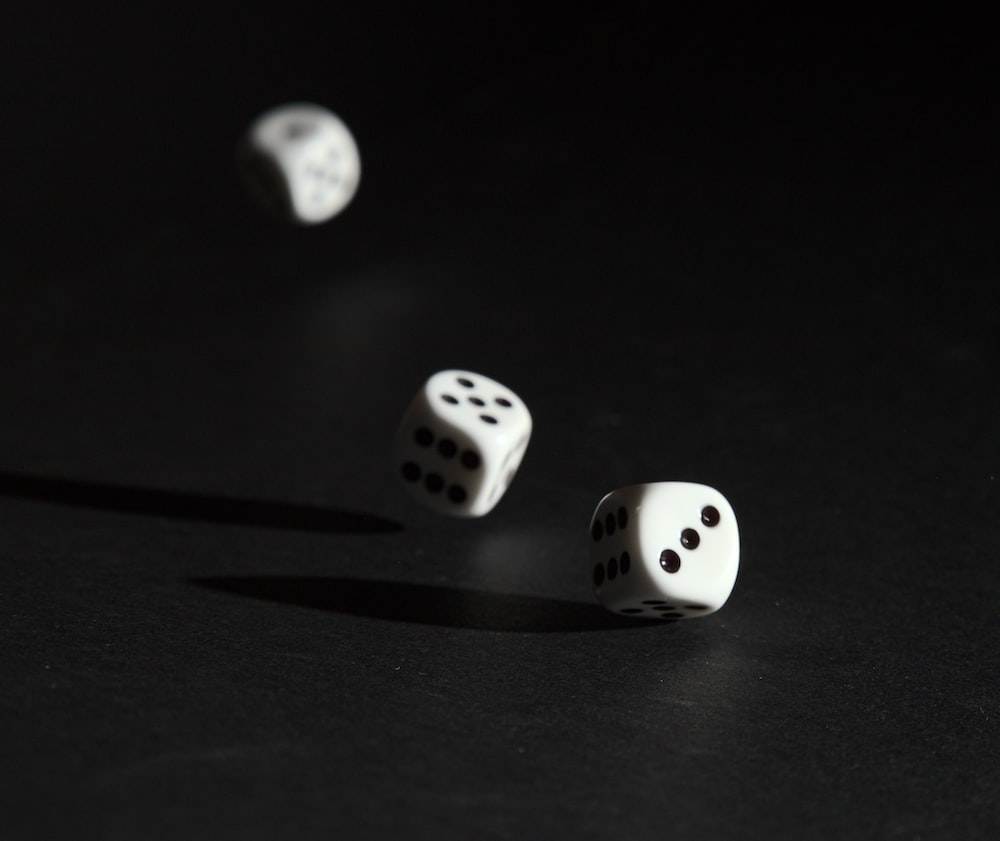
\includegraphics[scale = .055]{Images/dice2.jpg}

\includegraphics[scale = .6]{Images/coin_toss.jpg}
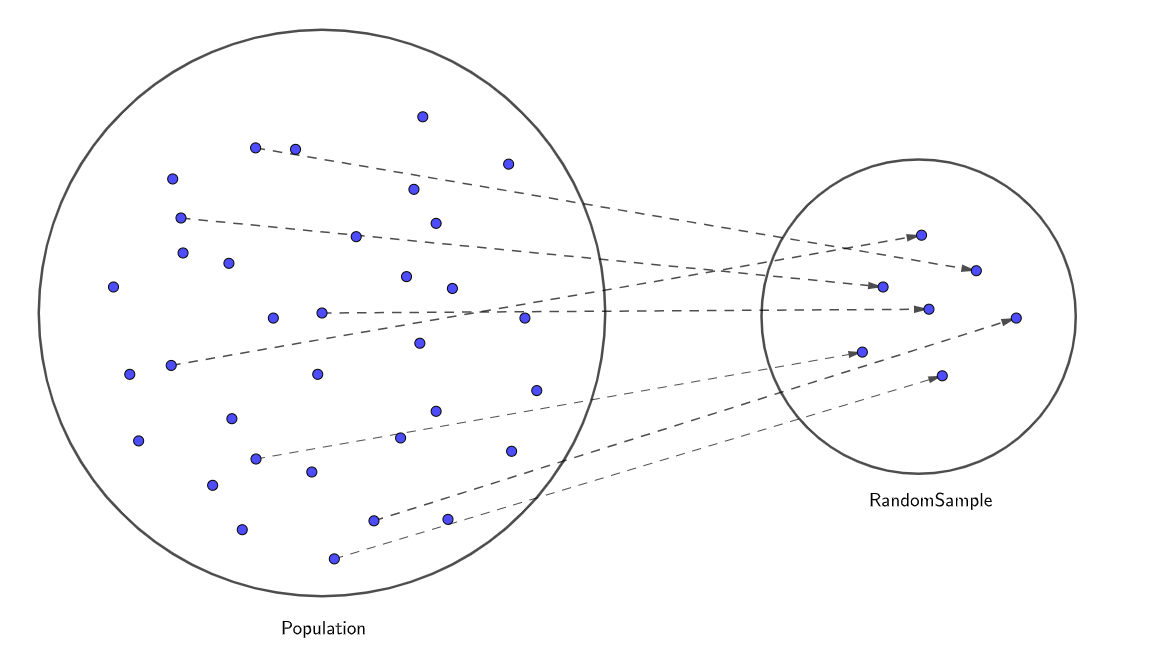
\includegraphics[scale = .1]{Images/Sampling.png}

\caption{Throwing dices, tossing a single coin and sampling from a population, all are examples of random experiment!}
\end{figure}




\item Once we know the sample space $\Omega$, we can actually form different subsets of $\Omega$, and think about different \alert{events}. Recall an \alert{events} is simply a subset of the sample space, so in principle everything that we have learned about Sets could be directly applicable when we are talking about Events. 

\framebreak

\item For example, for the coin toss experiment, when the sample space is $\Omega = \{\textrm{H}, \textrm{T}\}$, can you think about \alert{all possible events} (think about all possible subsets)? Yes, in this case, the answer is easy, it's the power set,


\begin{align*}
\mathcal{P}(\Omega) = \{  \{\textrm{H}\}, \{\textrm{T}\}, \{\textrm{H}, \textrm{T} \}, \emptyset  \}
\end{align*}


\begin{itemize}
\item $\{\textrm{H}\}$ is an event since $\{\textrm{H}\} \subset \Omega$. Here event $\{\textrm{H}\}$ means only head is appearing.
\item Similarly $\{\textrm{T}\}$ is an event, it means only tail is appearing.
\item $ \{\textrm{H}, \textrm{T}\} $ is also an event, since, it satisfies the definition of a subset. Note $\{\textrm{H}, \textrm{T} \} = \Omega$
\item {\color{red} Ques-} What does the event $ \{\textrm{H}, \textrm{T}\} $ mean? Ans: It means \emph{any one} of the outcomes will appear, we can write $\{\textrm{H}, \textrm{T} \}  = \{\textrm{H}\} \cup \{\textrm{T}\} $
\item It might look strange why $\emptyset$ is a subset of $\Omega$. The answer is, it satisfies the definition of a subset. Recall, the set A is a subset of the set B if and only if every / all element of A is also an element of B. If A is the empty set then A has no elements and so all of its elements (there are none) belong to B no matter what set B we have. So, the empty set $\emptyset$ is a subset of every set. And in this case $\emptyset \subset \Omega$. {\color{red} Ques-} \alert{What does the event $\emptyset$ mean?} Ans: It means, nothing is appearing, so it is an impossible event. 

\end{itemize}








\end{itemize}
\end{frame}
%---------------------------------------------------------------------------------


\section{Probability Definitions}
\frame{\sectionpage}

\begin{frame}[allowframebreaks]{Probability Definitions}


\begin{itemize}


\item Although all of us might have some intuitive understanding of probability, but the history of Mathematics tells us that the modern definition of probability came not so long ago.

\item  The Russian Mathematician Andrey Nikolaevich Kolmogorov (1903-87) laid the mathematical foundations of probability theory and the theory of randomness. 


\begin{figure}
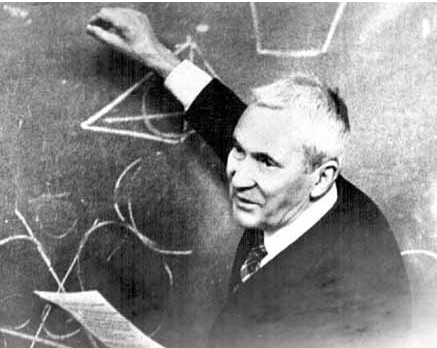
\includegraphics[scale = .4]{Images/kolmogorov1.png}
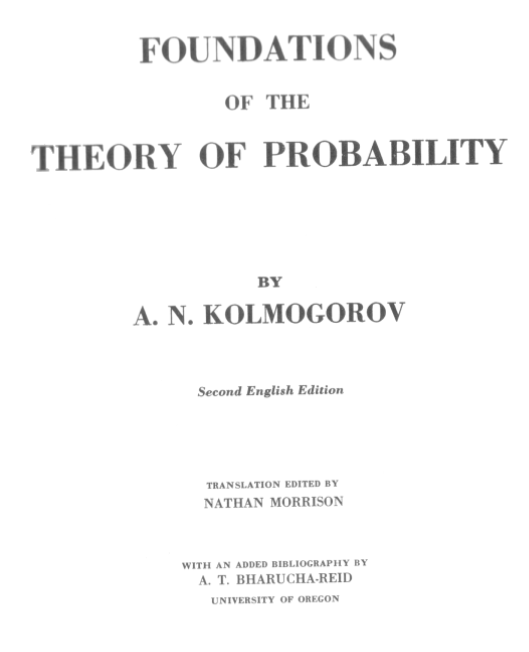
\includegraphics[scale = .2]{Images/kolmogorov_book.png}

\end{figure}


\item His monograph \alert{Grundbegriffe der Wahrscheinlichkeitsrechnung - Foundations of the Theory of Probability}\footnote[frame]{Go to \url{https://www.kolmogorov.com/Foundations.html} to see the scanned version of the English translation.}, published in 1933 first introduced the Probability Theory in a rigorous way using fundamental axioms. We will see the \alert{Axiomatic approach} of defining probability later, first let's see the \alert{Classical approach} and \alert{Frequentist approach} of defining probability.


\framebreak


\textbf{Important:}

\item In all definitions we will calculate probability for events as a function of events such that an event is an input and a probability is the output. 

\item For example if the set $A$ is an event (i.e., $A \subset \Omega$) then we will calculate the probability $\mathbb{P}(A)$ and this is going to be a number in $[0, 1]$.


\framebreak




\begin{varblock}{\Thm{Definition } - Classical Definition of Probability}

If an experiment has $n$ \alert{equally likely} outcomes, and there is an event $A$ where the number of outcomes is $n_A$, then the \alert{probability of the event $A$} is,

\begin{align}
\mathbb{P}(A) = \frac{n_A}{n}
\end{align}

\end{varblock}


\item So when we are thinking about the event $A$, the classical definition says we can calculate the probability by,

\begin{align*}
\mathbb{P}(A)=\frac{\text { number of outcomes in the event } A }{\text { number of outcomes in the sample space or total number of outcomes }}
\end{align*}

\framebreak

\item Let's apply the classical definition and calculate probabilities -
\medskip


\Thm{Example } 

Suppose our experiment is throwing a \alert{die}, and we want to know that \emp{what is the probability that the next outcome will be an even number?} Assume the die is a \emph{balanced die}, 

\medskip

First of all, note that here the word \emph{``balanced''} means all outcomes are \alert{equally likely}, so we can apply the classical definition. The sample space in this case is, $\Omega = \{1, 2, 3, 4, 5, 6 \}$, this means $n = 6$. Let $A$ be the event such that \alert{even number appears}, this means 

\begin{align*}
A = \{\omega: \omega \in \Omega \text{ and } \omega \text{ is an even number} \} = \{2, 4, 6 \}
\end{align*}


We want to calculate $\mathbb{P}(A)$. Here we have three outcomes for the event $A$ so $n_A = 3$, now applying the classical definition we get,

\begin{align*}
\mathbb{P}(A)= \frac{n_A}{n} = \frac{3}{6}=\frac{1}{2}
\end{align*}

\framebreak

\Thm{Example }
Suppose our experiment is tossing $2$ coins and assume that all the outcomes are equally likely (i.e., fair coins), now answer the following questions,


\medskip
\begin{itemize}
\item (a) What is the sample space $\Omega$?

\item (b) What is the probability of getting at least one head?


\end{itemize}

\bigskip

\Thm{Example } 

Now suppose the experiment is tossing $3$ coins, and assume that all the outcomes are equally likely (i.e., fair coins), now answer the following questions,



\medskip
\begin{itemize}
\item (a) What is the sample space $\Omega$?

\item (b) What is the probability of getting three heads?

\item (c) What is the probability of getting exactly one head and two tails?
\end{itemize}

\framebreak

{\Thm{Example }(This problem needs the knowledge of permutation or ordering concepts...)}

Suppose in a city license plates have six characters: $3$ letters followed by $3$ numbers, now answer the following questions,

\medskip

\begin{itemize}
\item a) How many distinct such plates are possible?
\item  b) How many distinct plates are possible if the license plate contains no duplicate letters or numbers?
\item c) Given that all sequences of six characters are equally likely, what is the probability that a randomly selected license plate for a new car will contain no duplicate letters or numbers?
\end{itemize}


\vspace*{.3cm}

\begin{itemize}
\item Ans of a) We can apply multiplication rule, there are $26^3=17,576$ different ways to choose the letters and $10^3=1000$ ways to choose the numbers, so we have $26^3 \times 10^3 = 17,576 \times 1000=17,576,000$ number of distinct plates. This means $\Omega$ consists the set of of all $17,576,000$ possible license plates, so here $n = 17,576,000$

\medskip
\item Ans of b) Let's denote the event with $A$ where we do not have any duplicates with numbers or digits. This means set $A$ has license plates with no duplicate letters or number. 
\medskip

Now, no duplicate letters means there are $26 \times 25 \times 24 = 15,600$ ways to choose the letters. And then, no duplicate numbers mean there are $10 \times 9 \times 8=720$ ways to choose the numbers. From the multiplication principle, the number of outcomes in the event $A$ is $15,600 \times 720=11,232,000$, so $n_A = 11,232,000$.
\medskip
\item Ans of c) So now we can calculate the probability of happening the event $A$,

$$
\mathbb{P}(A)=\frac{11,232,000}{17,576,000}=.64
$$
\end{itemize}


\framebreak

\medskip

\item We will solve more examples in the practice sheet, now let's discuss the issues with the classical definition.

\medskip



\item There are essentially two major problems with the classical definition of probability

\begin{itemize}
\item Assumption of equally likely outcomes (how do we know this?). For example if we have a biased coin, then how do we calculate probability.

\item Finite sample space issues (sample space can be very large, e.g., $\Omega = \mathbb{R}$)
\end{itemize} 


\item Another definition is known as the \alert{Frequency definition} of probability, let's see it now, this is a very important definition and we often use this to explain probability,



\framebreak


\begin{varblock}{\Thm{Definition } - Frequency Definition of Probability }

The probability of an event $A$ is the \emph{relative proportion of outcomes} if we perform the experiment \alert{under identical condition} for a \emph{large number of times}.

\end{varblock}

\item So for example if our experiment is tossing a single coin, the probability of appearing heads is the number of times heads will appear if we perform this experiment almost infinite number of times.

\item Any more example...

\framebreak

\item Frequency definition does not have equally likely outcomes assumption, but the issue is we need to perform the experiment \alert{under identical conditions}, and assume that we are performing many time.....this is often not possible.

\item Now we will see the axiomatic way to define probability, which doesn't have these issues. This is the most general way to define probability.


\item Important it's an \emph{abstract definition} where we will define probability as a \alert{set function} which will satisfy some rules, 


\item So we will set the rules that intuitively we think probability should satisfy, ...


\framebreak





\begin{varblock}{\Thm{Definition} - Axiomatic Definition of Probability}
For a random experiment, if we have a sample space $\Omega$ and then we can define probability as a \alert{set function} $\mathbb{P}(\cdot)$ such that for any event $A \subset \Omega$

\begin{itemize}
\item 1. $\mathbb{P}(A) \geq 0$ 
\item 2.  $\mathbb{P}(\Omega)=1$.
\item 3.  For \alert{pairwise disjoint but countable number of events} $A_1, A_2, \ldots$ we have

\begin{align*}
\mathbb{P}\left(A_1 \cup A_2 \cup A_3 \ldots \right)= \mathbb{P}\left(A_1\right) + \mathbb{P}\left(A_2\right) + \mathbb{P}\left(A_3\right) + \ldots
\end{align*}
\end{itemize}
\end{varblock}

\item[] \textbf{Sidenote: The idea of disjoint means,  $A_1 \cap A_2 = \emptyset$. In this case all possible pairs will be disjoint}


\item Let's explain each of these axioms (in class discussion).

\framebreak

\item Note that, unlike the other definition, the Axiomatic definition does not tell us any ways to calculate probabilities, it only defines probability as a function with some rules...

\item This means as long as any set function satisfies above three axioms, we will consider that function a probability function. Sometimes Probability function is also called \alert{Probability measure}. We won't talk about \emph{``measure''} in this course, but if some of you take advanced courses in probability theory, you will see this term. In fact probability function is called a measure.



\framebreak




\item With this definition, now we can show that the following rules of calculating probability 


\begin{varblock}{\Thm{Theorem } (Probability Calculus or Probability Rules)}
$\mathbb{P}(\cdot)$ is a probability function and $A$ and $B$ are any events, then we can show that

\begin{itemize}

\item a. $\mathbb{P}(\emptyset)=0$

\item b. $\mathbb{P}(A) \leq 1$

\item c. $\mathbb{P}\left(A^c\right)=1-\mathbb{P}(A)$

\item d. $\mathbb{P}(A \cup B)=\mathbb{P}(A)+\mathbb{P}(B)-\mathbb{P}(A \cap B)$;

\item e. If $A \subset B$, then $\mathbb{P}(A) \leq \mathbb{P}(B)$.

\end{itemize}

\end{varblock}



\textbf{Proof:} 

\textbf{c):}
\medskip

First using Venn diagram, we can see that 

\begin{align*}
\Omega = A \cup A^{\mathrm{c}}
\end{align*}

This means $A$ and $A^c$ makes a \emph{partition} of the sample space $\Omega$ (What is a partition? It simply means if we take union of disjoint sets will get the whole set) Now we will apply the axioms,

\begin{align*}
\Omega &= A \cup A^{\mathrm{c}} \\
\implies \mathbb{P}(\Omega) &= \mathbb{P}\left(A \cup A^c\right), \text{ [apply the second axiom] }\\
\implies  \mathbb{P}(\Omega) &= \mathbb{P}(A)+\mathbb{P}\left(A^{\mathrm{c}}\right) \text{ [$A$ and $A^c$ are disjoint, so apply the third axiom] } \\
\implies 1 &= \mathbb{P}(A)+\mathbb{P}\left(A^{\mathrm{c}}\right) \text{ [Apply first axiom] }
\end{align*}

So last line means  $\mathbb{P}\left(A^c\right)=1-\mathbb{P}(A)$. So we have shown $c$

\medskip
---------

\medskip
\textbf{b):}
\medskip

Since $0 \leq \mathbb{P}\left(A^{\mathrm{c}}\right) \leq 1$ and we know $	1 = \mathbb{P}\left(A^{\mathrm{c}}\right) + \mathbb{P}\left(A\right)$, it means we must have  $\mathbb{P}(A) \leq 1$, so this means (b) holds.

\medskip
---------
\medskip

\textbf{a):}
\medskip

To prove (a), we use a similar argument like $c$ First note, 

\begin{align*}
\mathbb{P}(\Omega \cup \emptyset)&=\mathbb{P}(\Omega)+\mathbb{P}(\emptyset) \text{ [ since $\Omega$ and $\emptyset$ are disjoint and $\Omega &= \Omega \cup \emptyset$, we apply third axiom ] }\\
\mathbb{P}(\Omega) &= \mathbb{P}(\Omega) + \mathbb{P}(\emptyset) \\
1 &= 1 + \mathbb{P}(\emptyset) \text{ [ apply second axiom ] }
\end{align*}

so we have $\mathbb{P}(\emptyset)=0$.

\framebreak

\textbf{d) and e):}
\medskip

Here we have 

\begin{align*}
  \mathbb{P}(A \cup B)=\mathbb{P}(A)+\mathbb{P}(B)-\mathbb{P}(A \cap B)
\end{align*}

and 

\begin{align*}
A \subset B, \text{ then } \mathbb{P}(A) \leq \mathbb{P}(B)
\end{align*}

We will not prove this in the class, but let's understand them visually. For proof you can look at \citet{casella_statistical_2002} (A bit advanced but a beautiful book!)



\qed 

\framebreak

\item As a side note here are the formal definitions of disjoint, pairwise disjoint and partition 

\begin{varblock}{\Thm{Definition } (Disjoint, Pairwise Disjoint and Partition)}

\begin{itemize}
\item Two events $A$ and $B$ are \alert{disjoint} (or also called \alert{mutually exclusive}) if $A \cap B=$ $\emptyset$. 

\item The sequence of events $A_1, A_2, \ldots$ are \alert{pairwise disjoint} (or \alert{pairwise mutually exclusive}) if $A_i \cap A_j=\emptyset$ for any $i \neq j$.


\item If $A_1, A_2, \ldots$ are pairwise disjoint and $\bigcup_{i=1}^{\infty} A_i=\Omega$, then the collection $A_1, A_2, \ldots$ forms a \alert{partition} of $\Omega$.

\end{itemize}


\end{varblock}

Partition means it will break the sample space in disjoint parts. These concepts are easy to understand if we draw the Venn Diagrams. 

\framebreak



\item $\mathbb{P}(A \cap B)$ is called the \emph{joint probability}, because this calculates the probability of happening both events. On the other hand $\mathbb{P}(A)$ and $\mathbb{P}(B)$ are called \emph{marginal probabilities}. 

\item Note that if $\mathbb{P}(A \cap B) = 0$, then $\mathbb{P}(A \cup B)=\mathbb{P}(A)+\mathbb{P}(B)$. But in general we cannot write this, we have to use Theorem 2.9 (d)




\framebreak






\item When we have a \alert{countable and finite sample space} then there is a nice rule to assign/calculate probability of an event $A$, following theorem gives us this rule. You have already applied this rule for the equally likely case. But now we don't need ``equally likely assumption''.

\begin{varblock}{\Thm{Theorem } (A rule to assign probabilities of events for a finite sample space)}

Let $\Omega=\left\{\omega_1, \ldots, \omega_n\right\}$ be a finite sample space and let $\mathbb{P}(\{\omega_i\}) = p_i$, for $ i = 1, 2, \ldots, n$  such that following two conditions hold 


\begin{align*}
\text{1. } &p_i \geq 0 \text{ for all }i = 1, 2, \ldots, n \\
\text{2. } &\sum_{i=1}^n p_i = 1
\end{align*}

If for any event $A$, we can define $\mathbb{P}(A)$ by

$$
\mathbb{P}(A)=\sum_{\left\{i: \omega_i \in A\right\}} p_i
$$

Also for $\emptyset$ we have $\mathbb{P}(\emptyset) = 0$, then we can show that $\mathbb{P}$ is a probability function (this means all axioms are satisfied).

\end{varblock}

The above theorem remains true if $\Omega$ is a countable set, it means we can apply this theorem when we have  $\Omega=\left\{\omega_1, \omega_2, \ldots\right\}$

\medskip

% \cite{anderson_statistics_2020} has the same rule in page 184. Note that \cite{anderson_statistics_2020} there is a slight abuse of notation, because it writes $\mathbb{P}(E_i)$, in principle it should be $\mathbb{P}(\{E_i\})$. This is abuse because in \cite{anderson_statistics_2020}, $E_i$ is an experimental outcome.


\framebreak


\item Let's see an application of this theorem. Suppose an experiment has five  outcomes: $\omega_1, \omega_2, \omega_3, \omega_4, \omega_5$ . Then if we know 

\begin{align*}
\mathbb{P}(\{\omega_1\}) = p_1 = 0.2 \\
\mathbb{P}(\{\omega_2\})= p_2 = 0.3 \\
\mathbb{P}(\{\omega_3\}) = p_3 = 0.2 \\
\mathbb{P}(\{\omega_4\}) = p_4 = 0.1\\
\mathbb{P}(\{\omega_5\}) = p_5 = 0.2 \\
\end{align*}

The theorem says we can calculate probabilities for any events. For example, we can calculate $P(\{\omega_1, \omega_2 \})$

\item First note the sample space is, $\Omega=\left\{\omega_1, \omega_2, \omega_3, \omega_4, \omega_5\right\}$. Now, let's calculate $P(\{\omega_1, \omega_2 \})$. If we apply the theorem we have,

\begin{align*}
P(\{\omega_1, \omega_2 \}) = p_1 + p_2 = 0.2 + 0.3 = 0.5
\end{align*}

\item Can you calculate the probability $P(\{\omega_1, \omega_2 \})$, if we assume equally likely assumption?

% \framebreak


% Let's see an example how to apply this theorem. Consider the simple experiment of tossing a coin, so $  \Omega=\{\mathrm{H}, \mathrm{T}\}$. Now we don't need to assume the coin is ``fair'', so in this case maybe we can define

% \begin{align*}
%   p_1 &= \mathbb{P}(\{\mathrm{H}\})=\frac{1}{9} \\
%   p_2 &= \mathbb{P}(\{\mathrm{T}\})=\frac{8}{9}
% \end{align*}

% Now, with this $p_1$ and $p_2$, we can calculate probabilities of any event. Think about an event and calculate the probability of happening that event. \alert{Ques:} What will be $p_1$ and $p_2$ if we assume ``equally likely'' experiment?


% \framebreak

% \medskip

% Ques: What will be $p_1$ and $p_2$ if we assume ``equally likely'' experiment? You know the answer. What if our sample space is infinite. Actually we don't know we need to verify the axioms in each case, and this might be very hard! There is a solution if we consider random variables....(more on this later!)


\end{itemize}

\end{frame}


%----------------------------------------------------------------
%----------------------------------------------------------------

\section{Conditional Probability}
\frame{\sectionpage}


\begin{frame}[allowframebreaks]{Conditional Probability}

\begin{itemize}


\item Now we will start with an new concept called \alert{Conditioning}. 


\item \emph{Conditioning is the soul of Statistics} (Joe Blitzstein, Harvard Stat 110)...



\item All of the probabilities that we have dealt so far are \alert{unconditional probabilities}. A sample space was defined and all probabilities were calculated with respect to that sample space. 

\item However in many instances, we have \emph{new information}, then if we calculate the probabilities with updated information, we call it \alert{Conditional Probability}, conditioning on that information.... 

\item Now, when we have new information, ideally we \emph{need to update the sample space}, however in many cases we are not in a position to \emph{update the sample space} and calculate probabilities. 

\item Hence the need for new tool, where we calculate the probabilities using the original sample space but with new information. Let's see the definition,

\framebreak


\begin{varblock}{\Thm{Definition } (Conditional Probability)}
If $A$ and $B$ are events in $\Omega$, and $\mathbb{P}(B)>0$, then the \alert{conditional probability} of $A$ given $B$ is defined as

\begin{align}
\mathbb{P}(A \mid B)=\frac{\mathbb{P}(A \cap B)}{\mathbb{P}(B)}
\end{align}



\end{varblock}

\framebreak

\item Let's see an example

\medskip
\Thm{Example } (Conditional Probability)

\item Suppose we have a data of recently admitted $150$ students from the four Departments (BBA, EEE, CSE and ECO) of EWU. We also have information whether before taking the admission, they tried to go abroad for undergrad or not (recall this is just a contingency table or cross-tabulation). 

\medskip

\begin{table}
\centering
\begin{tabular}{|lccccc|}
\hline & \multicolumn{4}{c}{ Departments } & \\
\cline { 2 - 6 }  & BBA & EEE & CSE & ECO & Total \\
\hline Tried & 18 & 13 & 22 & 24 & 77 \\
Not Tried & 22 & 25 & 16 & 10 & 73 \\
\hline Total & 40 & 38 & 38 & 34 & 150 \\
\hline
\end{tabular}
\end{table}

\framebreak

% Imipramine BBA
% Lithium ECO
% Combination CSE
% Placebo ECO

% Relapse Tried
% No Relapse Not Tried

\item Here are couple of questions (For all questions assume, equally likely case, this means all students have same probability of being selected)

\medskip

Following questions are for a randomly selected student from the $150$ students that we have....

\medskip

\begin{itemize}
\item a) What is the probability that a randomly selected student had tried abroad?

\medskip

\item b) What is the probability that a randomly selected student studies at the ECO Department?

\medskip

\item c) What is the probability that a randomly selected student studies at the ECO Dept. and also had tried abroad?

\medskip

\item d) \emph{If we know that the student is from ECO}, what is the probability that a randomly selected student had tried abroad? 

\medskip


\item[] \textbf{Note:} In future, often we will omit the phrase \emph{``randomly selected''}... but whenever there is a question about probability, it means we are talking about a random experiment. 


\end{itemize}
\medskip

\framebreak

\item Note in this case, the random experiment is selecting a random student from the $150$ students

\item The sample space is the set of all $150$ students

\item Now we answer the questions one by one, first let's define


\begin{itemize}

\item Let $A$ be the event that the student had tried abroad. 

\item Let $B$ be the event that the student is from the ECO Department. 

\end{itemize}


\medskip

\item The first question asks us to calculate $\mathbb{P}(A)$, the second question asks us to calculate $\mathbb{P}(B)$, the third question asks us to calculate $\mathbb{P}(A \cap B)$, and the fourth question asks us to calculate $\mathbb{P}(A|B)$

\framebreak

\item We calculate applying classical definition (this is what we will usually do in these problems)

\begin{align*}
\mathbb{P}(A) = \frac{\# \text{ of students who had tried abroad} }{\# \text{ total students} } = \frac{77}{150} \\
\\
\mathbb{P}(B) = \frac{\# \text{ of students who studies at ECO} }{\# \text{ total students} } = \frac{34}{150}
\end{align*}



\item So far  we calculated the \emph{marginal probabilities} of $A$ and $B$. 

\item Now we can also calculate the \alert{joint probability} $\mathbb{P}(A \cap B)$, here $A\cap B$ is the event where a randomly selected student studies at ECO and also had tried abroad.  

\begin{align*}
\mathbb{P}(A \cap B) = \frac{24}{150}
\end{align*}


\framebreak


\item Now we calculate the \emph{conditional probability}, here we apply the formula for $\mathbb{P}(A | B)$, 

\begin{align*}
\mathbb{P}(A|B) = \frac{\mathbb{P}(A \cap B)}{\mathbb{P}(B)} = \frac{24/150}{34/150} = \frac{24}{34}
\end{align*}

\item Note that there is a difference between the joint event $A \cap B$ and the conditional event $A \mid B$


\medskip

\item Interesting to note is, the conditional probability can also be calculated directly from the cell values using


\begin{align*}
 \frac{\# \text{ From the ECO students who had tried abroad} }{\# \text{Total ECO students} } = 24/34
\end{align*}

this is the calculation with the \emph{updated sample space} that includes only ECO students

\medskip

\item In this case we don't need to apply the formula $\mathbb{P}(A|B) = \frac{\mathbb{P}(A \cap B)}{\mathbb{P}(B)} $, we can directly do the calculation as,


\item The conditional formula for $\mathbb{P}(A|B)$ is there when we would like to use the original sample space and we want to calculate the conditional probability. ..






\framebreak
\item We can also calculate $\mathbb{P}(A^c|B) = 1 - \mathbb{P}(A|B) = 10/34$. This is always possible for conditional probability.

\item So conditional probability function will act like a probability function. But it will give us an updated calculation with respect to the new sample space. 


\item So you can say that, the intuition of conditional probability calculation is - our original sample space $\Omega$ has been updated to $B$, and then all further calculations are updated with respect to their relation to $B$. 

\framebreak

\item \textbf{Two Important Questions:}


\item \textbf{Ques 1}: What happens to conditional probabilities of disjoint sets? 


\item Ans: Let $A$ and $B$ are disjoint, so $A \cap B = \emptyset$. Note in this case, $\mathbb{P}(A \cap B)=0$. So $\mathbb{P}(A \mid B)=\mathbb{P}(B \mid A)=0$. This means conditional probability of disjoint sets is always $0$. So conditioning on $B$ will not give any information about $A$ if $A$ and $B$ are disjoint. 


\medskip

\item \textbf{Ques 2:} When do we have $\mathbb{P}(A \mid B) = \mathbb{P}(A)$ 

\item Ans: Note that this happens when $\mathbb{P}(A \cap B) = \mathbb{P}(A) \times \mathbb{P}(B)$, since

\begin{align*}
 	\mathbb{P}(A \mid B) = \frac{\mathbb{P}(A \cap B)}{\mathbb{P}(B)} = \frac{\mathbb{P}(A) \times \mathbb{P}(B)}{\mathbb{P}(B)} = \mathbb{P}(A)
 \end{align*} 

\item It means conditional and unconditional probabilities are same ... we will come back to this later... actually this happens when $A$ and $B$ are independent events.


\framebreak

\item Now note that the conditional probability definition gives a way to calculate the probabilities of a joint event, using the formula in (2), we get,


\begin{align}
\mathbb{P}(A \cap B) = \mathbb{P}(A | B) \mathbb{P}(B)
\end{align}

\item This is sometimes called \alert{the multiplication rule of conditional probability} (do not confuse this with the multiplication rule for counting!)

\item Now using the same idea in (2) we can also calculate

\begin{align}
\mathbb{P}(B \mid A)=\frac{\mathbb{P}(A \cap B)}{\mathbb{P}(A)}, \text{ given that } \mathbb{P}(A) \neq 0
\end{align}

\item From here using the multiplication idea, we get

\begin{align*}
\mathbb{P}(A \cap B) = \mathbb{P}(B | A) \mathbb{P}(A)
\end{align*}


\item So now we have a different way of writing $\mathbb{P}(A | B)$,

\begin{align}
\mathbb{P}(A | B) = \frac{\mathbb{P}(A \cap B)}{\mathbb{P}(B)} = \frac{\mathbb{P}(B | A) \mathbb{P}(A)}{\mathbb{P}(B)} 
\end{align}

\item The last formula where we ``turned around'' the conditional probabilities is called \alert{Bayes' Rule}, this is after the name of Sir Thomas Bayes.

\item So the Baye's Rule is 


\begin{varblock}{\Thm{Theorem } (Bayes' Rule)}
Let $A$ and $B$ be two events on the sample space $\Omega$, and assume that $\mathbb{P}(B)>0$, then we have


\begin{align}\label{BayesRule}
\mathbb{P}(A | B) = \frac{\mathbb{P}(B | A) \mathbb{P}(A)}{\mathbb{P}(B)} 
\end{align}

\end{varblock}

\begin{figure}[H]
\centering
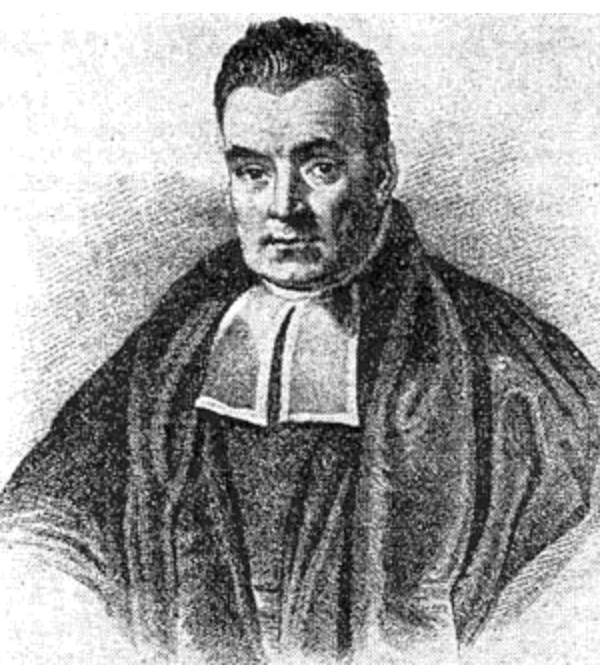
\includegraphics[scale = .2]{Images/Bayes.png}
  
\end{figure}









\framebreak

\item Note for three sets $A_1, A_2, A_3$ using Conditional Probability we can also calculate,

\begin{align*}
\mathbb{P}(A_3 \mid A_1 \cap A_2) = \frac{\mathbb{P}(A_1 \cap A_2 \cap A_3)}{\mathbb{P}(A_1 \cap A_2)}
\end{align*}

\item Using the multiplication rule of conditional probability, we get

\begin{align*}
\mathbb{P}(A_1 \cap A_2 \cap A_3) &= \mathbb{P}(A_1 \cap A_2) \times \mathbb{P}(A_3 \mid A_1 \cap A_2) \\
&= \mathbb{P}(A_1) \times \mathbb{P}(A_2 | A_1) \times \mathbb{P}(A_3 \mid A_1 \cap A_2) 
\end{align*}

\item You can extend this formula for more than $2$ events, but I am skipping the general version, see \citet*{degroot_probability_2012} for details.

% \begin{align*}
% \mathbb{P}(A_1 \cap A_2 \cap A_3 \cap \, , \ldots, \cap A_n) &= \mathbb{P}(A_1) \times \mathbb{P}(A_2 | A_1) \\
% &\times \mathbb{P}(A_3 \mid A_1 \cap A_2) \times \mathbb{P}(A_4 \mid A_1 \cap A_2 \cap A_3 ) \times  \\
% &\ldots,  \times \mathbb{P}(A_n \mid A_1 \cap A_2 \cap A_3 \cap,\ldots, \cap A_{n - 1})
% \end{align*}


\framebreak

\item Now we will learn another law, which is called \alert{Law of Total Probability}. This law is very important and it is an application of \emph{partition}. 


\begin{varblock}{\Thm{Theorem } (Law of Total Probability )}
Let $A_1, \ldots, A_n$ be events that form a partition of the sample space $\Omega$  and assume that $\mathbb{P}\left(A_i\right)>0$, for all $i$. Then, for any event $B$, we have


\begin{align}\label{eq:LTP}
\mathbb{P}(B)&=\mathbb{P}\left(B \mid A_1\right)\mathbb{P}\left(A_1\right) +\cdots+ \mathbb{P}\left(B \mid A_n\right)\mathbb{P}\left(A_n\right) 
\end{align}
\end{varblock} 



\item We will skip the general proof, but let's understand the theorem for a simpler case.

\framebreak

\item Consider the following Venn diagram, 

\begin{figure}[H]
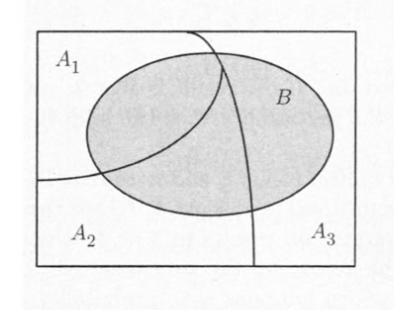
\includegraphics[scale = .4]{Images/LTP.png}
\end{figure}

\item Here $A_1, A_2 \text{ and } A_3$ forms a  \emph{partition}. Recall a partition is a sequence of sets which splits the entire sample space.

\item If $A_1$, $A_2$ and $A_3$ forms a partition of $\Omega$ and $B$ is a set, then we can write,

\begin{align}
B=\left(A_1 \cap B\right) \cup \left(A_2 \cap B\right) \cup \mathbb{p}\left(A_3 \cap B\right)
\end{align}

\item All sets are disjoint, so using the axiom we have,

\begin{align*}
\mathbb{P}(B)=\mathbb{P}\left(A_1 \cap B\right)+ \mathbb{P}\left(A_2 \cap B\right) + \mathbb{P}\left(A_3 \cap B\right)
\end{align*}


\item Now using conditional probabilities we have


\begin{align*}
\mathbb{P}(B)&=\mathbb{P}\left(A_1 \cap B\right)+ \mathbb{P}\left(A_2 \cap B\right) + \mathbb{P}\left(A_3 \cap B\right) \\
&= \mathbb{P}\left(B \mid A_1\right)  \mathbb{P}\left(A_1\right)+  \mathbb{P}\left(B \mid A_2\right) \mathbb{P}\left(A_2\right) + \mathbb{P}\left(B \mid A_3\right) \mathbb{P}\left(A_3\right) 
\end{align*}


\item So this is the Law of Total Probability, but we explained it for three sets. You can extend the idea generally for $n$ sets,


\begin{align*}
\mathbb{P}(B) = \mathbb{P}(B \mid A_1) \mathbb{P}(A_1) + \cdots + \mathbb{P}(B \mid A_n) \mathbb{P}(A_n) 
\end{align*}




\framebreak

\item It is possible to apply the Bayes' rule here. First note applying simple Bayes' rule for set $A_1$ and $B$ we get,



\begin{align*}
\mathbb{P}\left(A_1 \mid B\right) &=\frac{\mathbb{P}\left(A_1\right) \mathbb{P}\left(B \mid A_1\right)}{\mathbb{P}(B)}
\end{align*}

\medskip

\item Now we apply the law of total probability for $\mathbb{P}(B)$

\medskip

\begin{align*}
\mathbb{P}\left(A_1 \mid B\right) &=\frac{\mathbb{P}\left(A_1\right) \mathbb{P}\left(B \mid A_1\right)}{\mathbb{P}(B)} \\
&=\frac{\mathbb{P}\left(A_1\right) \mathbb{P}\left(B \mid A_1\right)}{\mathbb{P}\left(B \mid A_1\right)\mathbb{P}\left(A_1\right)+\cdots+\mathbb{P}\left(B \mid A_n\right)\mathbb{P}\left(A_n\right) }
\end{align*}

\item This is what we call the general version of the Bayes' rule or the Bayes' rule with law of total probability.

\item Now we write the general version.

\framebreak



\begin{varblock}{\Thm{Theorem } (Bayes' Rule with Law of Total Probability)}
Let $A_1, A_2, \ldots, A_n$ be events that form a partition of the sample space $\Omega$, and assume that $\mathbb{P}\left(A_i\right)>0$, for all $i$. Then, for any event $B$ such that $\mathbb{P}(B)>0$, we have


\begin{align*}
\mathbb{P}\left(A_i \mid B\right) &=\frac{ \mathbb{P}\left(B \mid A_i\right) \mathbb{P}\left(A_i\right)}{\mathbb{P}(B)} \\
&=\frac{\mathbb{P}\left(A_i\right) \mathbb{P}\left(B \mid A_i\right)}{\mathbb{P}\left(B \mid A_1\right)\mathbb{P}\left(A_1\right)+\cdots+\mathbb{P}\left(B \mid A_n\right)\mathbb{P}\left(A_n\right) }
\end{align*}


\end{varblock}



\end{itemize}

\end{frame}



% \section{More Problems}

% \begin{frame}{More Problems on Conditioning}

% \Thm{Example } (Problem on Conditioning)

% Suppose we have the following test results for a class of students. There are only two possible Grades, Grade A or Grade B, otherwise students fail the course. The course is offered combinedly for Bachelor and Master level students. We have the following data. 


% \begin{align*}
% &\begin{array}{lc|ccc|c} 
% \hline & \multicolumn{5}{c}{ \text{\sc Grades} }  \\
% \cline { 2 - 6 } & & A_1 & A_2 & A_3 & \text { Totals } \\
% \cline { 2 - 6 } \text { \sc Level } &  B_1  & 352 & 197 & 251 & 800 \\
% \text {  } & B_2  & 150 & 161 & 194 & 505 \\
% \cline { 2 - 6 } \text { \sc  } & \text { Totals } & 502 & 358 & 445 & 1305
% \end{array}
% \end{align*}


% Note in the table $A_1$, $A_2$ and $A_3$ means Grade $A$, $B$ and $F$ and $B_1$, $B_2$ means Masters and Bachelors students. 



% \end{frame}


% \begin{frame}{More Problems on Conditioning}

% \begin{itemize}
% \item Calculate the joint probabilities and write down in a table. 

% First Calculate each of the joint probabilities, and plug the value in the table. Here is the joint probability table

% \begin{align*}
% &\begin{array}{lc|ccc|c} 
% \hline & \multicolumn{5}{c}{ \text{\sc Grades} }  \\
% \cline { 2 - 6 } & & A_1 & A_2 & A_3 & \text { Totals } \\
% \cline { 2 - 6 } \text { \sc Level } &  B_1  & 0.27 & 0.15 & 0.19 & 0.61 \\
% \text {  } & B_2  & 0.12 & 0.12 & 0.15 & 0.39 \\
% \cline { 2 - 6 } \text { \sc  } & \text { Totals } & 0.39 & 0.27 & 0.34 & 1
% \end{array}
% \end{align*}

% \item Given that a student is a Bachelor student what is the Probability that he got grade $A$?
% \item Given that a student failed what is the Probability that he is a Masters student?
% \end{itemize}

% \end{frame}


% \begin{frame}{More Problems on Conditioning}

% \Thm{Example } (Bayes Rule and Conditioning)

% Now suppose we change the question a bit. We don't know the joint table of numbers of joint probability table but we have following information. 

% We know $61\%$ are Master student and $39\%$ are Bachelor students. Out of the Master students, $44\%$ got A,  $25\%$ got B and $31\%$ Failed. So with this information only find out given if the student got A, what is the probability that he is a Master student.


% In this case, we are asking, $\mathbb{P}(B_1 \mid A_1)$.  


% \end{frame}

\section{Independence}
\frame{\sectionpage}



\begin{frame}[allowframebreaks]{Independence}

\begin{itemize}

\item The idea of independent events is very easy, we need to check whether joint probability is same as the product of marginal probability.


\begin{varblock}{\Thm{Theorem } (Independence of two events)}
Let $A$ and $B$ be two events from the sample space $\Omega$, we say $A$ and $B$ are independent if 

\begin{align*}
\mathbb{P}(A \cap B) = \mathbb{P}(A) \times \mathbb{P}(B)
\end{align*}


\end{varblock}

\item Here is one interpretation, since multiplication of probabilities will always be smaller, you can think when the events are independent than their joint probability will be very small.


\item The idea of independence can also be explained via the conditional probability. This is what we mentioned in page 77. Recall, when $A$ and $B$ are independent we have


\begin{align*}
 	\mathbb{P}(A \mid B) = \frac{\mathbb{P}(A \cap B)}{\mathbb{P}(B)} = \frac{\mathbb{P}(A) \times \mathbb{P}(B)}{\mathbb{P}(B)} = \mathbb{P}(A)
 \end{align*} 


\item So the unconditional probability or the marginal probability of $A$ is same as the conditional probability. So learning $B$ makes no difference to the probability of $A$.


\framebreak

\item We can easily extend this concept to more than two events, the idea is then we need all subsets of the events to be independent.

\item As an example, in order for three events $A, B$, and $C$ to be independent, the following four relations must be satisfied:

$$
\begin{aligned}
&\mathbb{P}(A \cap B)=\mathbb{P}(A) \mathbb{P}(B) \\
&\mathbb{P}(A \cap C)=\mathbb{P}(A) \mathbb{P}(C) \\
&\mathbb{P}(B \cap C)=\mathbb{P}(B) \mathbb{P}(C)
\end{aligned}
$$
and
$$
\mathbb{P}(A \cap B \cap C)=\mathbb{P}(A) \mathbb{P}(B) \mathbb{P}(C)
$$

\item This idea is what we call \alert{mutual independence}.



\begin{varblock}{\Thm{Definition } (Independent Events).}
The $k$ events $A_1, \ldots, A_k$ are independent (or mutually independent $)$ if, for every subset the joint probability of the events can be written as a product of marginal probabilities.
\end{varblock}

\item You will see some problems in the problem set.


\end{itemize}

\end{frame}







\begin{frame}[allowframebreaks]{References}
\vspace*{.3cm} 

\scriptsize
% \printbibliography[maxnames=99]

% \nocite{*}
\bibliographystyle{apalike}
\bibliography{../common/references}  
% \nocite{*}

\end{frame}

\end{document}
